
	\subsection{Circuito completo}
		\graficarEPS{0.6}{banco_med_full}{Diagrama del circuito para mediciones con etapa de potencia.}{fig:banco_med_full}
		A continuación se presentan las mediciones realizadas durante la semana del \texttt{18/02/2019}. Se realizó el conexionado del circuito de modo tal que se tiene el circuito completo como se muestra en la Figura \ref{fig:banco_med_full}. 

		%\section{Cambios durante las mediciones}
			%Cortocircuitamos el inductor y la carga en su lugar posta.

			%Medicion slew rate: entramos con \SI{200}{\mV} y \SI{250}{\mV} y frecuencai \SI{1}{\kHz}.

%
%		\subsubsection{Respuesta en frecuencia}
%
		\subsubsection{Impedancia de salida}

		Para la medición de la resistencia de salida se utilizó el banco de medición de la Figura \ref{fig:bco_zo} con una resistencia de prueba de \SI{8}{\ohm} y un capacitor de \SI{10}{\micro\farad}. Se utilizaron varias frecuencias, obteniéndose las Figuras \ref{fig:zo_100} y \ref{fig:zo_10k}.

		\begin{figure}[h!]
			\centering
			\includegraphics[width=0.8\textwidth]{./Mediciones/Zo_100}
			\caption{Medición de la impedancia de salida a \SI{100}{\Hz}.}
			\label{fig:zo_100}
		\end{figure}
		\begin{figure}[h!]
			\centering
			\includegraphics[width=0.8\textwidth]{./Mediciones/Zo_10k}
			\caption{Medición de la impedancia de salida a \SI{10}{\kHz}.}
			\label{fig:zo_10k}
		\end{figure}


\begin{figure}[H]
	\centering
	\includegraphics[scale=0.5]{./Figuras/bco_zo_salida.eps}
	\caption{Banco de medición. Impedancia de salida.}
	\label{fig:bco_zo}
\end{figure}

A partir de las mediciones realizadas, el valor de $R_o$ en función de las tensiones máximas medidas es \eqref{eq:zo_med}

\begin{equation}
	\centering
	\hat{v}_1 = \frac{R_p}{R_o + R_p} \implies R_o = \frac{R_p \cdot (\hat{v}_1 - \hat{v}_2)}{\hat{v}_1}
	\label{eq:zo_med}
\end{equation}


Los resultados obtenidos se resumen en la Figura \ref{fig:zo_med}

\begin{figure}[H]
	\centering
	\includegraphics[scale=0.5]{./Figuras/med_zo.pdf}
	\caption{Resistencia de salida.}
	\label{fig:zo_med}
\end{figure}

	Aunque la forma de la curva de la Figura \ref{fig:zo_med} se asemeje a la simulada (Figura \ref{fig.sim_ro} no pueden ser comparadas dado que la medición se encuentra con errores propios de no poder utilizar valores más pequeños de resistencia para hacer la comparación y hallar el valor verdadero.

\subsubsection{Ancho de banda de potencia}

Utilizando el mismo banco de medición de la ganancia, se analizó la variación de la frecuencia de corte en función de la potencia disipada en la carga, obteniéndose la Tabla \ref{tab.bw_pote}.

\begin{table}[H]
	\centering
	\begin{tabular}{cccc}
		\toprule
		Potencia [W] & 1 & 10 & 40 \\
		\midrule
		Frecuencia [\SI{}{\kilo\hertz}] & 153,8 & 153 & 120 \\
		\bottomrule
	\end{tabular}
	\caption{Ancho de banda de potencia.}
	\label{tab.bw_pote}
\end{table}

	En esta ocasión, los valores de $BW$ son más próximos a los simulados que los calculados con el circuito sin potencia. Ésto puede deberse principalmente a que, al tratarse de grandes potencias, el circuito requiera dicha etapa para poder operar de manera esperada.
%
%		\subsubsection{Margen de fase}
%
	\pagebreak
	
		\subsubsection{\emph{Slew-Rate}}
		Se mide a máxima potencia y a $\SI{1}{\kHz}$ y se calcula la pendiente a la salida que se genera por la respuesta al escalón. Dicho valor seasemeja al valor esperado por el análisis previo.
	

		\begin{figure}[H]
			\centering
			\includegraphics[scale=0.1]{./Mediciones/SlewRatePotencia.jpg}
			\caption{Slew Rate.}
		\end{figure}

		\begin{equation*}
			SR  = \frac{\varDelta v}{\varDelta t} = 11.213 \frac{V}{us}
		\end{equation*}

		\subsubsection{Respuesta en frecuencia}

		\begin{figure}[H]
			\centering
			\includegraphics[width=0.8\textwidth, trim = 0 160 0 160]{./Figuras/bw_total.pdf}
			\caption{Respuesta en frecuencia a 1W.}
		\end{figure}


		
		\subsubsection{Variación de la Fuente de Alimentación}
		Al variar la fuente de alimentación entre -25 y 33 V, se miden los distintos puntos de polarizacion, tal que las corrientes de polarización no varien mas de un 10 por ciento.
		\begin{table}[]
			\centering
		\begin{tabular}{|l|l|l|l|l|l|l|l|l|l|l|}
		\hline
		Vcc{[}V{]} & -Vcc{[}V{]} & A{[}V{]} & B{[}V{]} & C{[}V{]} & D{[}V{]} & E{[}V{]} & F{[}mV{]} & G{[}mV{]} & H{[}V{]} & I{[}mV{]} \\ \hline
		30.11      & 30          & 12.36    & 1.369    & -29.07   & 1.31     & -1.275   & 27.3      & 11.8      & 29.43    & 10.6      \\ \hline
		31.22      & 30.99       & 12.39    & 1.364    & -29.68   & 1.308    & -1.271   & 25.5      & 7.6       & 30.57    & 10.5      \\ \hline
		32.71      & 32.56       & 12.4     & 1.362    & -31.24   & 1.310    & -1.275   & 27.2      & 10.6      & 32.06    & 10.6      \\ \hline
		24.98      & 25          & 12.06    & 1.358    & -23.69   & 1.309    & -1.270   & 24.6      & 6.3       & 24.37    & 9.9       \\ \hline
		26.99      & 27.02       & 12.18    & 1.363    & -25.7    & 1.309    & 1.27     & 26.1      & 9.6       & 26.37    & 10.3      \\ \hline
		28.39      & 28.18       & 12.25    & 1.363    & -26.86   & 1.311    & -1.27    & 27.1      & 10.2      & 27.75    & 9.2       \\ \hline
		29.21      & 29.13       & 12.29    & 1.363    & -27.82   & 1.311    & -1.275   & 26.2      & 10.4      & 28.58    & 9.3       \\ \hline
		\end{tabular}
		\caption{Valores de polarización ante variaciones de $V_{CC}$}
		\label{tab.valores}
		\end{table}



		En el Figura \ref{fig:esq_med} se marcan los puntos correspondientes a las mediciones de polarización de la Tabla \ref{tab.valores}.

		\begin{figure}[H]
			\centering
			\includegraphics[scale=0.6]{./Figuras/esquema_puntos.pdf}
			\caption{Puntos de medición.}
			\label{fig:esq_med}
		\end{figure}
			
		Se calcula la corriente sobre cada componente de importancia
		\begin{equation*}
		I_i = \frac{V_n - V_{n-1}}{R_i} 
		\end{equation*}

		\begin{table}
			\centering
		\begin{tabular}{|l|l|l|l|}
		\hline
		Parámetro & Valor de polarización & Maxima variación & Variación Porcentual \\ \hline
		$I_{R12}$      & \SI{4.99}{\mA}       		  & \SI{4.864}{\mA}		&  2.5 \\ \hline
		$V_{BE}$      & \SI{2.585}{\V}      		  & \SI{2.579}{\V}		& 0.02  \\ \hline
		$I_{R6}$      & \SI{6.8}{\mA}      		  & \SI{6.4}{\mA}		& 5.88  \\ \hline
		\end{tabular}
		\end{table}

		
		\subsubsection{Distorsión total armónica}

		El banco de medición para la distorsión total armónica se muestra en la Figura \ref{fig:thd_bco}. Los valores se obtuvieron mediante el software \textit{SpectraPlus}. Se utilizó la placa de audio de la PC para generar la señal, ya que un generador de laboratorio presenta un valor elevado de \texttt{THD}. Asimismo es necesario utilizar un atenuador resistivo debido a que la PC no admite como entrada un valor mayor a 1Vrms. 

		\begin{figure}[h!]
			\centering
			\includegraphics[scale=0.6]{./Figuras/banco_thd.eps}
			\caption{Banco de medición de \texttt{THD}.}
			\label{fig:thd_bco}
		\end{figure}

		\begin{figure}[H]
			\centering
			\includegraphics[scale=0.6]{./Figuras/thd.pdf}
			\caption{THD en función de la frecuencia.}
			\label{fig:thd}
		\end{figure}

		\begin{figure}[H]
			\centering
			\includegraphics[scale=0.6]{./Figuras/thd_zoom.pdf}
			\caption{THD en función de la potencia.}
		\end{figure}

		\subsubsection{Distorsión por intermodulación}

		De manera análoga a la simulación, se calculó la IMD mediante el \textit{software SpectraPlus} con el mismo banco de medición que la Figura \ref{fig:thd_bco}. Las mediciones se realizaron a \SI{5}{\kilo\hertz} para las potencias \SI{0.1}{\watt}, \SI{1}{\watt}, \SI{10}{\watt}

			\begin{table}[H]
				\centering
				\begin{tabular}{cc}
				\toprule
				Potencia [W] & IMD [\%]\\
				\midrule
				0,1 & 0.0593 \\
				1 & 0,0254 \\
				10 & 0,0127 \\
				40 & 0,0253 \\
				\bottomrule
				\end{tabular}
				\caption{Distorsión por intermodulación.}
			\end{table}
			%\Flor{Valores para 100 y 5kHz como la simulación. Tambien está 60 7k hecha}



		\subsubsection{Relación Señal a Ruido}
		Para realizar la medición de la SNR se utilizó el programa Spectra Plus en el cual se midio con ruido blanco para geerar el piso que presenta la placa de sonido y luego se generó una señal a $\SI{1}{\kHz}$ y $\SI{1}{\W}$ midiendo la salida con el banco de medición de la Figura \ref{fig:thd_bco} .



			\begin{figure}[H]
				\centering
				\includegraphics[scale=0.6]{./Figuras/ruido_balnco.jpg}
			\caption{Piso de ruido.}
			\end{figure}

			\begin{figure}[H]
				\centering
				\includegraphics[scale=0.6]{./Figuras/SNR_1K_1W_imagen2.jpg}
			\caption{Salida a \SI{1}{\W} y \SI{1}{\kHz}.}
			\end{figure}


			Calculando:

			\begin{equation*}
			SNR_{db}  = 20 \, \log\left(\frac{V_{ruido}}{V_o}\right) = V_{ruido_{dB}} - V_{o_{dB}}
			\end{equation*}

			Por lo tanto: 

			\begin{equation*}
				SNR_{db}  = 98.75 - 8.21 = \SI{90.54}{\dB}  
			\end{equation*}
	


		\subsubsection{Máxima excursión de salida}
		Se introdujo una señal de amplitud (máxima) tal que la salida no recorte. Dicha señal corresponde a una
		de amplitud pico a pico 2.14 $V_{pp}$. A la salida se obtiene $V_{pp}$ = 50 V. El banco de medición se muestra en la Figura \ref{fig:bco_ganancia}. Sin embargo, cabe destacar que durante la medición de eficiencia del circuito, se logró una tensión de salida $V_{pp} = \SI{53}{\V}$ coincidiendo con el valor simulado cercano a \SI{26}{\V}. De todas formas la potencia que se alcanza en ambos casos es mayor a \SI{40}{\W} que era lo que se pretendía.

		\begin{figure}[h!]
			\centering
			\includegraphics[scale=0.5]{Figuras/bco_ganancia.eps}
			\caption{Medición de máxima excursión de salida antes del recorte.}
			\label{fig:bco_ganancia}
		\end{figure}

		\begin{figure}[h!]
			\centering
			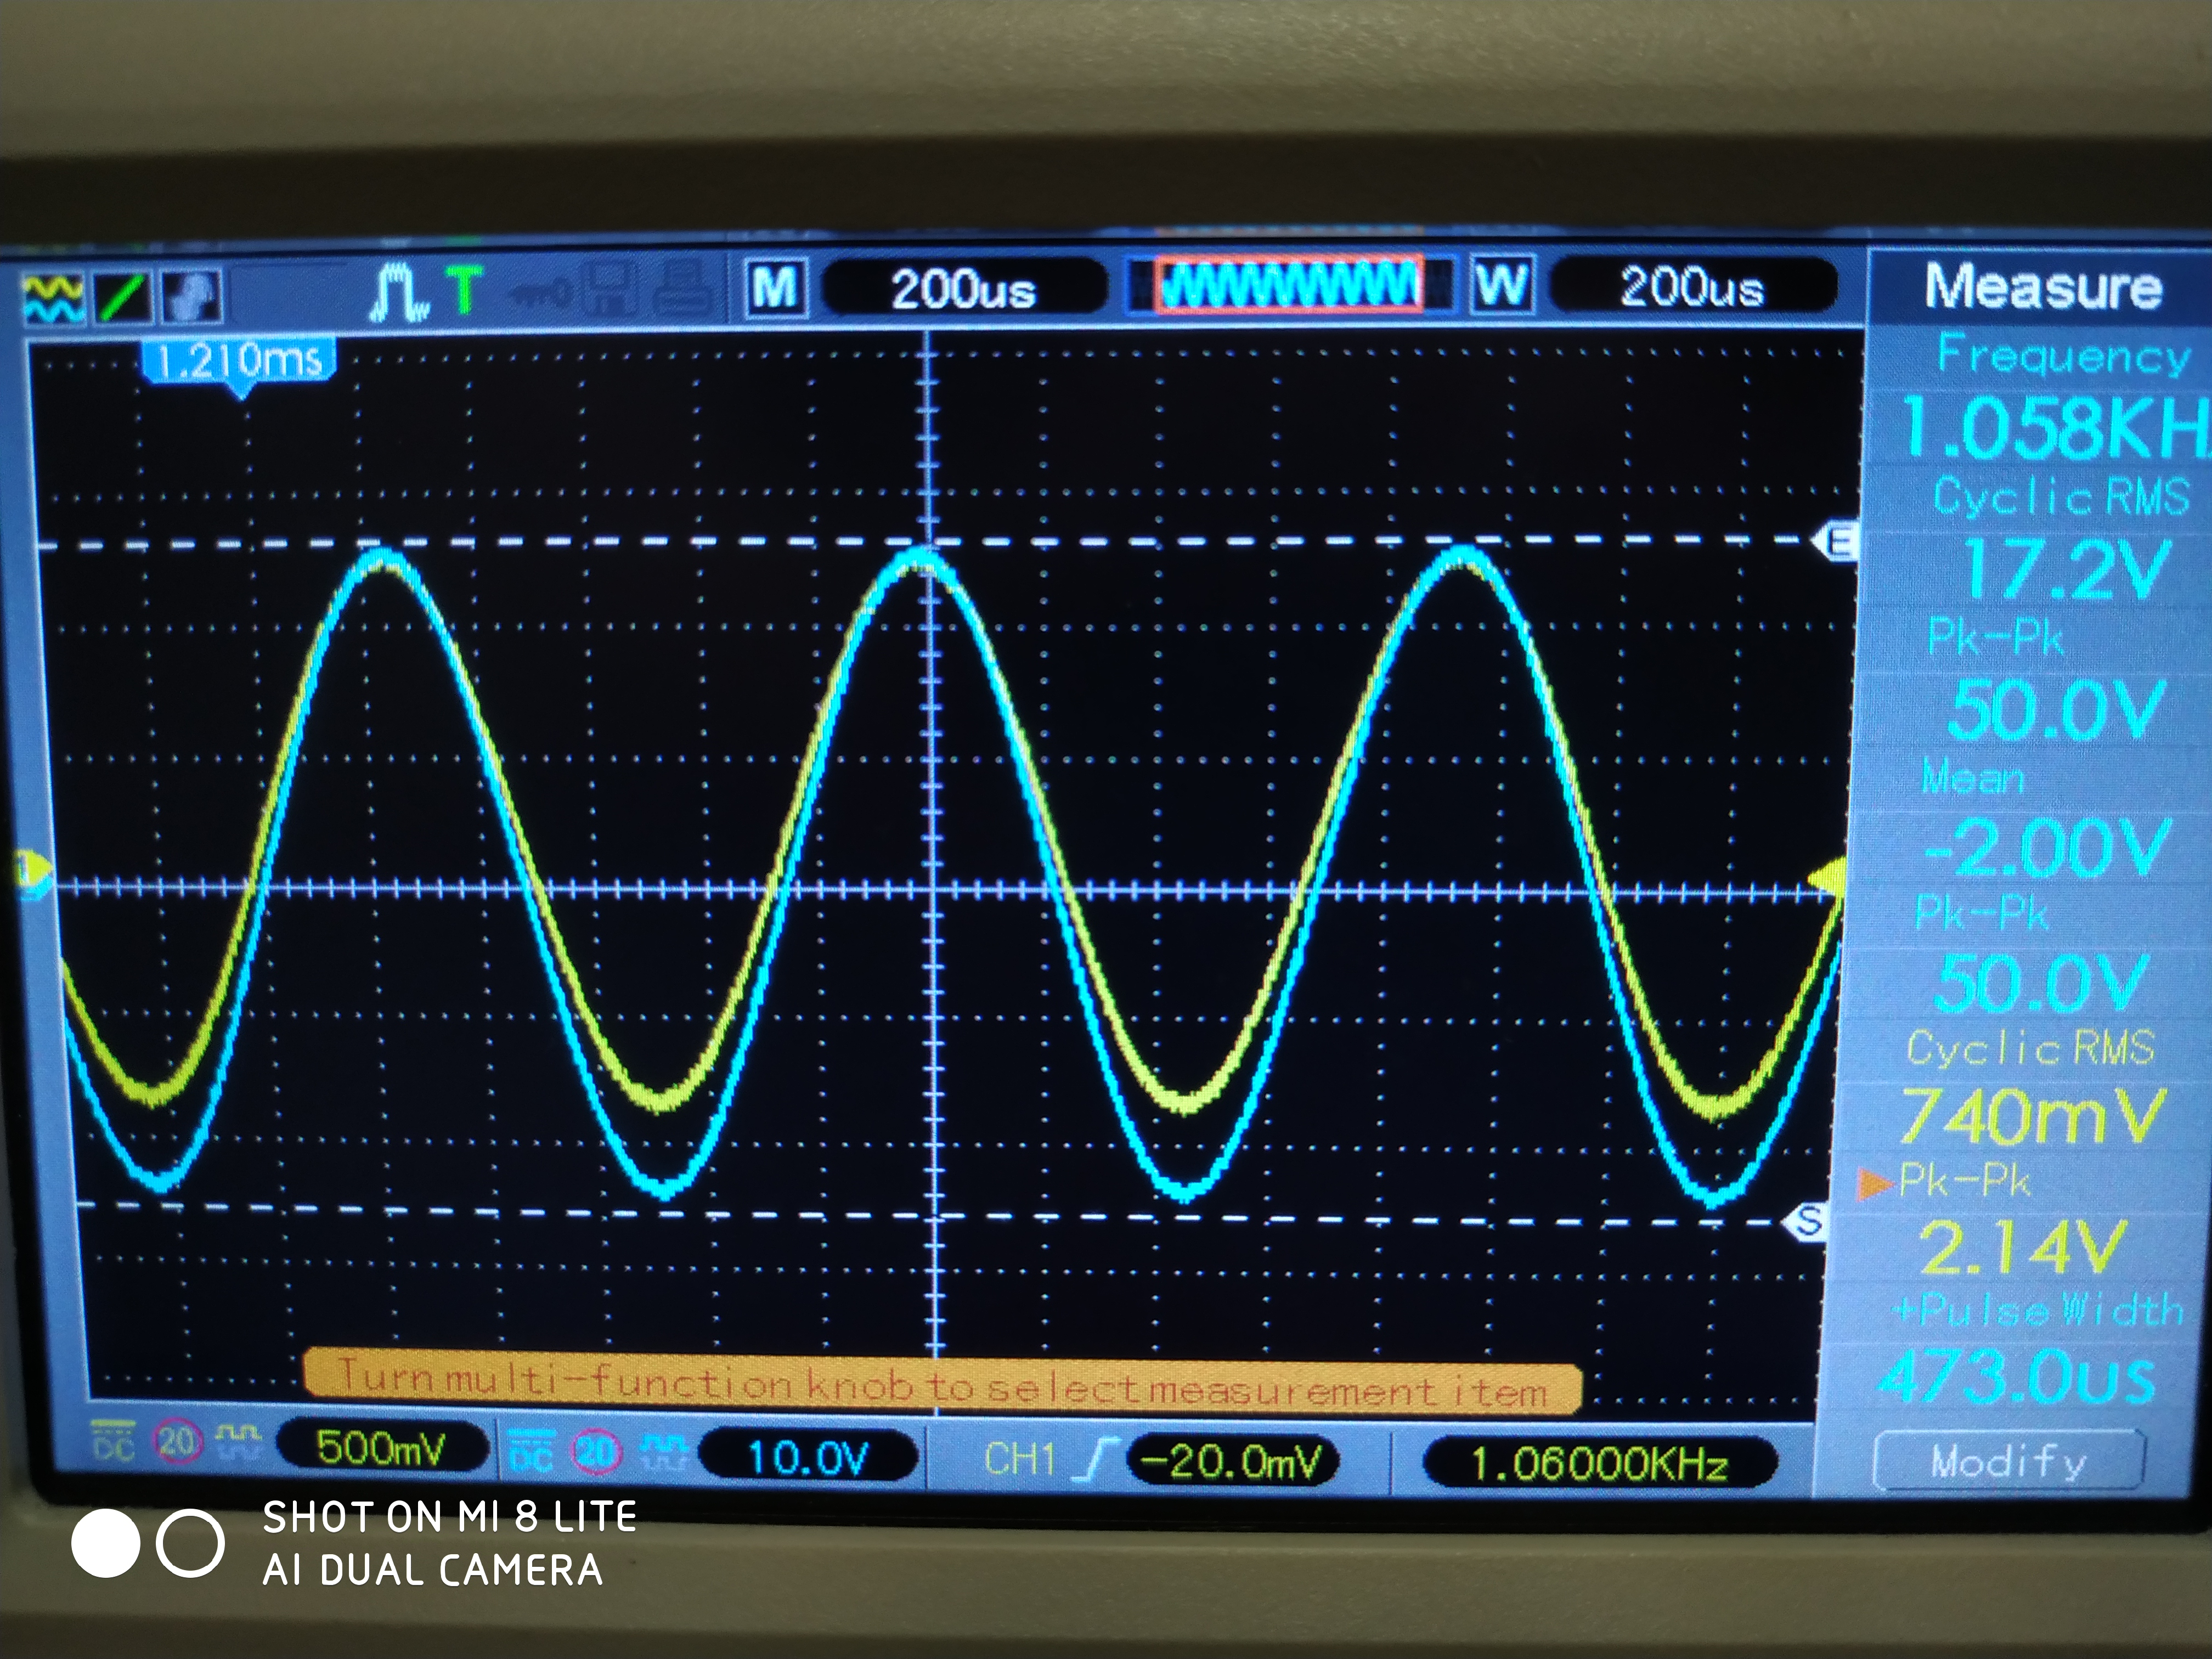
\includegraphics[scale=0.1]{Mediciones/PotenciaMaxima.jpg}
			\caption{Medición de máxima excursión de salida antes del recorte.}
			\label{fig:MaxExcur}
		\end{figure}


%%%%%%%%%%%%%55
%		\subsubsection{Rechazo de Ruido de la Fuente de Alimentación}
%%%%%%%%%%%%%%%%%%%

		\subsubsection{Máxima eficiencia del amplificador}
			\graficarEPS{1.0}{graf_eficiencia_vs}{Eficiencia en función de la potencia disipada por la carga para \SI{100}{\Hz}, \SI{1}{\kHz} y \SI{10}{\kHz}}{fig:eficiencia}
			Los amplificadores clase G se caracterizan por la eficiencia que poseen para señales de pequeña amplitud. Como se ve en la Figura \ref{fig:eficiencia}, para potencias disipadas por la carga menores a \SI{7}{\W} (en un amplio rango de frecuencias), la eficiencia del circuito crece con una pendiente 10 veces mayor que la de un clase B tradicional. Sin embargo, para potencias mayores el circuito la eficiencia se comporta como un clase B teniendo una relación proporcional a la potencia.

			Los valores de eficiencia máximos son de 70\% para $\hat{v}_o=\SI{10.4}{\V}$ y \SI{26.5}{\V}.


	\subsubsection{Comportamiento térmico}
		También se midió la temperatura del disipador con el multímetro para el caso de máxima potencia. Los resultados en función del tiempo se muestran en la Tabla \ref{tab.temp}. Luego de aproximadamente un minuto, la temperatura no presentó variaciones notables. 

\begin{table}[H]
	\centering
	\begin{tabular}{cccccc}
	\toprule
		Temperatura [\SI{}{\degree}C] & 33 & 33 & 34 & 35 & 38 \\
		\midrule
		Tiempo [s] & 5 & 17 & 46 & 54 & 70 \\
		\bottomrule
	\end{tabular}
	\caption{Temperatura en la salida ($T_{ambiente}= \SI{27}{\degree}C$).}
	\label{tab.temp}
\end{table}



